\hypertarget{seccion:IniciarSesion}{\vspace{1pt}}
\section{Marco Teórico}

\subsection{Big Data}
El término Big Data se refiere a cantidades enormes de información, por ejemplo, la cantidad de información que se produce todos los días con el uso de una red social como Facebook, o la cantidad de datos que producen computadoras y dispositivos electrónicos que se auto monitorean mediante sensores. Esos volúmenes masivos de datos pueden ser utilizados para extraer conocimiento de ellos, y posteriormente atacar problemas que no sería posible resolver sin el Big Data.

\subsubsection{Las 3 Vs del Big Data}

\begin{enumerate}
	\item \textbf{Volumen:} Con Big Data, se tendrán que procesar grandes volúmenes de información de baja densidad y sin estructura.
	\item \textbf{Velocidad:} Qué tan rápido se leen o se procesan los datos.
	\item \textbf{Variedad:} Múltiples tipos de datos y de archivos que se pueden procesar con el uso de Big Data.
\end{enumerate}

\subsubsection{Casos de uso del Big Data}

\begin{UClist}
	\UCli \textbf{Desarrollo de productos:} Compañías como Netflix y Procter \& Gamble utilizan el Big Data para anticiparse a la demanda de los consumidores de sus productos. Utilizan modelos predictivos para sus nuevos productos clasificando atributos clave de sus anteriores productos modelando las relaciones entre esos atributos.
	\UCli \textbf{Mantenimiento predictivo:} Se pueden predecir fallas mecánicas en maquinaria que de otra forma quedarían fácilmente ignoradas. Mejorando así ampliamente la calidad y el costo del mantenimiento de dichos equipos.
	\UCli \textbf{Experiencia de usuario:} El uso de Big Data permite recopilar toda la información sobre el usuario y utilizarla a favor de su experiencia en un sitio o aplicación. Por ejemplo, sus búsquedas frecuentes, los sitios que visita, etc. Para de esta manera empezar a hacerle ofertas o anuncios personalizados, según sus intereses particulares.
	\UCli \textbf{Machine Learning:} Actualmente el machine learning es un área de mucho auge, ya que permite entrenar a las computadoras mediante conjuntos de datos de entrenamiento en lugar de programarlas. El Big Data facilita esa tarea.
\end{UClist}

\subsection{Minería de datos}
La minería de datos es el proceso de detectar la información procesable de los conjuntos grandes de datos. Utiliza el análisis matemático para deducir los patrones y tendencias que existen en los datos. Normalmente, estos patrones no se pueden detectar mediante la exploración tradicional de los datos porque las relaciones son demasiado complejas o porque hay demasiado datos.
Estos patrones y tendencias se pueden recopilar y definir como un modelo de minería de datos. Los modelos de minería de datos se pueden aplicar en escenarios como los siguientes:
\begin{UClist}
	\UCli \textbf{Pronóstico:} Cálculo de las ventas y predicción de las cargas del servidor o del tiempo de inactividad del servidor.
	\UCli \textbf{Riesgo y probabilidad:} Elección de los mejores clientes para la distribución de correo directo, determinación del punto de equilibrio probable para los escenarios de riesgo, y asignación de probabilidades a diagnósticos y otros resultados.
	\UCli \textbf{Recomendaciones:} Determinación de los productos que se pueden vender juntos y generación de recomendaciones.
	\UCli \textbf{Búsqueda de secuencias:} Análisis de los artículos que los clientes han introducido en el carrito de la compra y predicción de posibles eventos.
	\UCli \textbf{Agrupación:} Distribución de clientes o eventos en grupos de elementos relacionados, y análisis y predicción de afinidades.
\end{UClist}

\subsection{Árboles de decisión}
Un árbol de decisión es una representación de una función multivariada y que fue posible utilizar de manera práctica a partir del desarrollo de las computadoras modernas. El interés por el uso práctico de los árboles de decisión tuvo su origen las necesidades de las ciencias sociales.\\

Los árboles de decisión están formados por los siguientes elementos:

\begin{UClist}
	\UCli \textbf{Nodos:} Nombres o identificadores de los atributos.
	\UCli \textbf{Ramas:} Posibles valores del atributo asociado al nodo.
	\UCli \textbf{Hojas:} Conjuntos ya clasificados de ejemplos y etiquetados con el nombre	de una clase. 
\end{UClist}

\pagebreak
\begin{figure}[!htbp]
	\hypertarget{fig:arbol-decision-ejemplo}{\hspace{1pt}}
	\begin{center}
		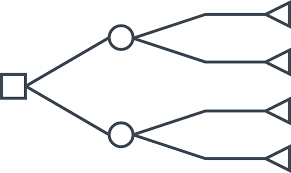
\includegraphics[height=0.3\textheight]{capitulo2/images/arbol-decision-ejemplo.png}
		\caption{Representación general de un árbol de decisión}
		\label{fig:arbol-decision-ejemplo}
	\end{center}
\end{figure}

Quinlan (1986) desarrolló el algoritmo \nameref{id3} este utiliza la medida de entropía de la información para crear los árboles. Este fue mejorado y fue denominado \nameref{c4.5} por su autor Quinlan (1993).\\

A continuación se dará una breve descripción de los algoritmos \nameref{id3} y \nameref{c4.5}.

\subsubsection{ID3 (Iterative Dichotomiser 3)} \label{id3}
Este algoritmo construye un árbol de decisión que mantenga cada instancia de la secuencia de datos de entrada lo más compacta posible. Estos datos de enrtada se toman a partir de una tabla llamada \textbf{tabla de inducción}.\\

Una característica importante a destacar de este algoritmo es que el árbol de decisión que se genera es útil para aproximar una función objetivo de valores \textbf{discretos} utilizando la \textbf{entropía}.\\

El resultado de la ejecución de este algoritmo puede expresarse como un conjunto de reglas \textbf{\textit{si-entonces}}.\\

Los datos de entrada del algoritmo son los siguientes:\\

\begin{UClist}
	\UCli \textbf{Atributos:} Son los factores que influencian la clasificación o decisión. La selección de estos atributos debe basarse en el conociento acumulado por la experiencia. Cada atributo forma un nodo intermedio en un árbol cuyas hojas o nodos terminales son las clases o decisiones.
	\UCli \textbf{Clase:} Posible valor de solúción.
	\UCli \textbf{Conjunto de ejemplos:} Conjunto de combinaciones de atributos dados. Dado este conjunto, el ID3 selecciona el atributo que subdivide los ejemplos \textit{de la mejor manera}.
	\UCli \textbf{Entropía:} La entropía es la medida de la incertidumbre que hay en un sistema. Es decir, ante una determinada situación, la probabilidad de que ocurra cada uno de los posibles resultados. La entropía máxima que se puede tener es 1, la mínima es 0.\\

Este parámetro se calcula con la siguiente fórmula:

\pagebreak
\begin{figure}[!htbp]
	\hypertarget{fig:formula-entropia}{\hspace{1pt}}
	\begin{center}
		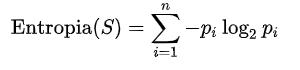
\includegraphics[width=0.3\textwidth, height=0.07\textheight]{capitulo2/images/formula-entropia.png}
		\caption{Fórmula para calcular la entropía}
		\label{fig:formula-entropia}
	\end{center}
\end{figure}
\end{UClist}

\subsubsection{C4.5} \label{c4.5}

\subsection{Spark}
Es una herramienta de código abierto. Es un motor de análisis de datos unificado para Big Data y Machine Learning. 
\subsection{Hadoop}
Es un framework de software que soporta aplicaciones distribuidas bajo una licencia libre. Permite a las aplicaciones trabajar con miles de nodos y petabytes de datos. Hadoop se inspiró en los documentos Google para MapReduce y Google File System (GFS). Hadoop utiliza su propio sistema de archivos HDFS, que divide archivos grandes y los distribuye en diferentes nodos para su procesamiento.
% Para que la ELD pueda mantener actualizado el status de pago de los aspirantes que realizaron la operación en sucursal bancaria, es necesario que el \textbf{Contador General} actualice de forma manual dichos pagos, esto se logra con ayuda del archivo brindado por BANAMEX, el cual servirá para ser cargado en el sistema y este lo interprete y determine si es correcto, en caso de ser correcto actualizar el estado de pago de los aspirantes que allí se encuentran, de lo contrario mostrar las inconsistencias.\\
% Una de las operaciones que brinda el sistema, es la actualización manual del status de pago de un aspirante, esta acción le permite tener el control para la actualización del status de pago de los aspirantes, esto con la finalidad de no depender del archivo de BANAMEX en caso de que presentaran conflictos con el mismo.
%\subsubsection{Procedimiento}
\begin{enumerate}
	\item Solicite administrar los pagos admisión seleccionando la opción \textbf{Administración de pagos} del menú \refIU{fig:menuPrincipalCG}{Menú del Contador General} y posteriormente la opción \textbf{Pagos Admisión} del menú \refIU{fig:menuPagosA}{Menú Pagos Admisión}.
	\item Se mostrará la pantalla \refIU{fig:APA}{Administrar Pagos Admisión}.
	\begin{figure}[!htbp]
		\hypertarget{fig:APA}{\hspace{1pt}}
		\begin{center}
			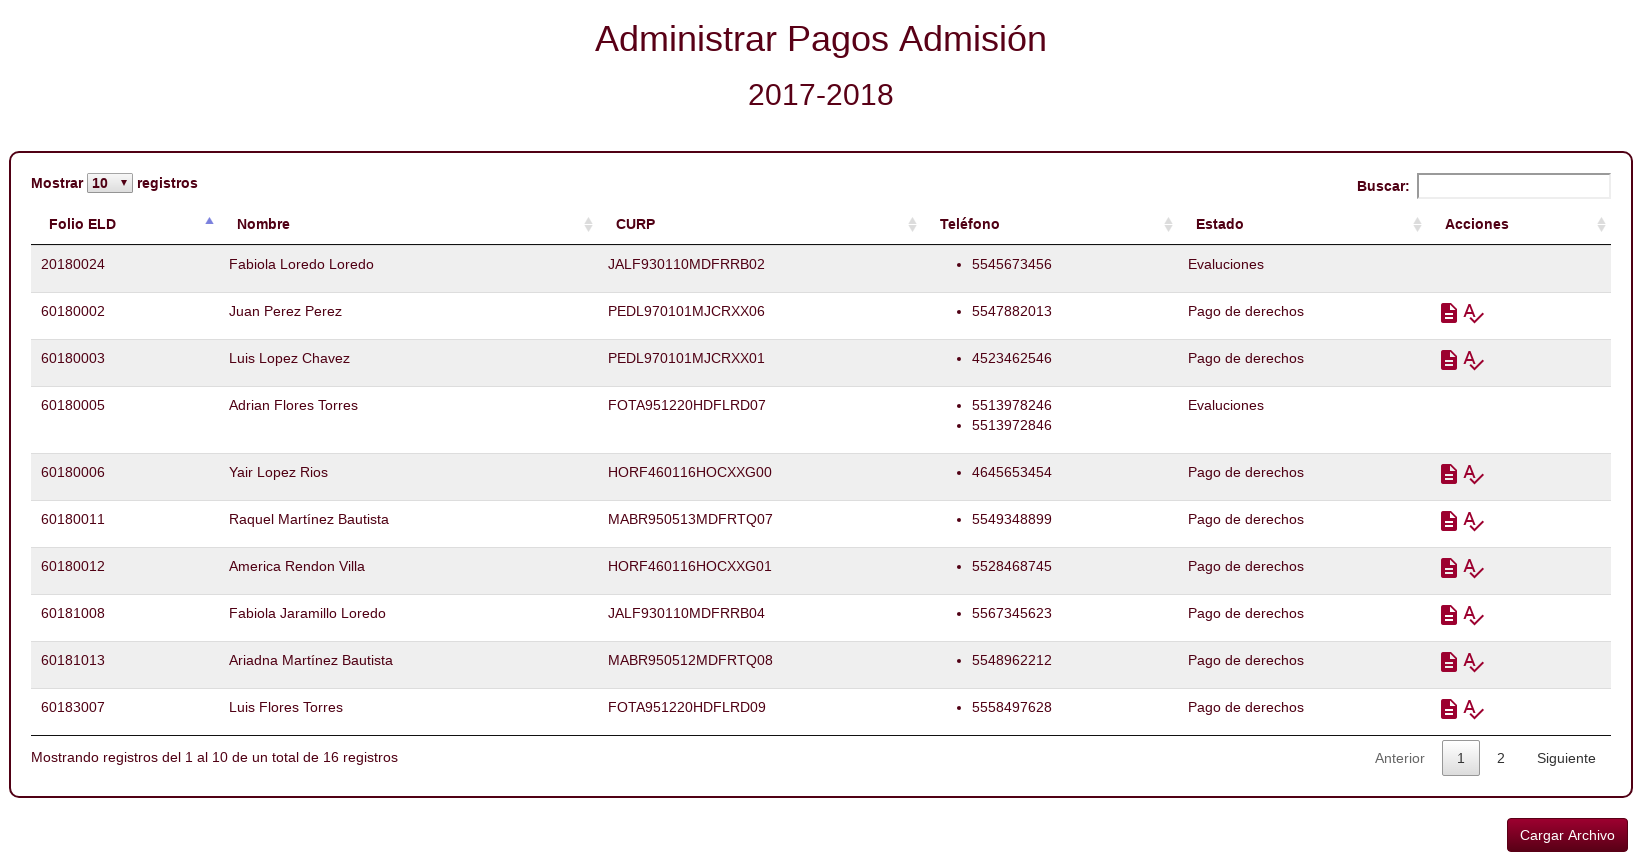
\includegraphics[height=0.3\textheight]{capitulo1/images/IU-APA.png}
			\caption{Administrar Pagos Admisión}
			\label{fig:APA}
		\end{center}
	\end{figure}

	
\end{enumerate}
	


\newpage
\begin{Errores}
	\error{El sistema muestra un mensaje indicando que falta información para realizar la operación.}
	{
		\begin{UClist}
			\UCli	Verifique que exista una convocatoria \textbf{Publicada}.
			\UCli	Verifique que exista un periodo de pagos.
			\UCli	Verifique que exista un periodo de pre-registro CENEVAL vigente.
		\end{UClist}
	}
	\error{El sistema muestra un mensaje indicando que no se ha realizado la asociación de fechas de CENEVAL y Psicométrico.}
	{
		\begin{UClist}
			\UCli	Verifique que la Coordinación de Control Escolar haya asociado las fechas CENEVAL y Psicométrico.
		\end{UClist}
	}
	

\end{Errores}
